\chapter{Calculations}

\section{Average density matrix}\label{apx:average-density}

The series expansions of the Casimir terms in the PFA $1/(\mathscr{L}^i_{A(B)})^2$ from eq. \eqref{eq:4:L-casimir} are given by:
\begin{multline}
  \frac{1}{(\mathscr{L}^i_{A(B)})^2} \approx \frac{4}{(d-2L+2R)^2} \pm \frac{8 \Delta x_{A(B)}\sin\delta}{(d-2L+2R)^3}
  \pm \theta_{A(B)}\left(\frac{8\Delta x_{A(B)} \cos\delta}{(d-2L+2R)^3}\right) \\
  + L_{A(B)}\left(\frac{16}{(d-2L+2R)^3} \pm \frac{48\Delta x_{A(B)} \sin\delta}{(d-2L+2R)^4}\right) \pm \theta_{A(B)}L_{A(B)}\frac{48\Delta x_{A(B)} \cos\delta}{(d-2L+2R)^4}
\end{multline}
where again the abbreviation $\delta = \alpha,\beta$ was used and the $\pm$ terms align to the corresponding notation in eq. \eqref{eq:4:L-casimir}. The series expansion for the gravitational terms $1/L^{ij}$ with $i,j = 1,2$ from eq. \eqref{eq:4:L-gravity} is given by
\begin{multline}
  \frac{1}{L^{ij}} = \frac{1}{2L} \pm \frac{\Delta x_B \sin\beta - \Delta x_A \sin\alpha}{8L^2} \mp \theta_A\frac{\Delta x_A\cos\alpha}{8L^2} \pm \theta_B\frac{\Delta x_B\cos\beta}{8L^2} \\
  + L_A \left(-\frac{1}{4L^2} \pm \frac{\Delta x_A \sin\alpha-\Delta x_B \sin\beta}{8L^3}\right)
  + L_B \left(-\frac{1}{4L^2} \pm \frac{\Delta x_A \sin\alpha-\Delta x_B \sin\beta}{8L^3}\right) \\
  \pm L_A \theta_A \frac{\Delta x_A \cos\alpha}{8L^3} \mp L_A \theta_B \frac{\Delta x_B \cos\beta}{8L^3}
  \pm L_B \theta_A \frac{\Delta x_A \cos\alpha}{8L^3} \mp L_B \theta_B \frac{\Delta x_B \cos\beta}{8L^3} \\
  + L_A L_B \left(\frac{2}{4L^3} \pm \frac{3\Delta x_B \sin\beta - 3 \Delta x_A \sin\alpha}{16L^4}\right) \\
  \mp L_A L_B \theta_A \frac{3 \Delta x_A \cos\alpha}{16L^4} \pm L_A L_B \theta_B \frac{3 \Delta x_B \cos\beta}{16L^4}
\end{multline}
The resulting average over $\theta_{A(B)}$ and $L_{A(B)}$ can be computed by
\begin{equation}\label{eq:apx:average-density-element}
  \int_{-\infty}^{\infty} \dd \theta_A \dd \theta_B \dd L_A \dd L_B \, p(\theta_A) p(\theta_B) p(L_A) p(L_B) e^{i \phi}
\end{equation}
where $p(\,\cdot\,)$ is a gaussian probability distribution in the form of
\begin{equation}
  p(x) = \frac{1}{\sqrt{2\pi}\Delta x} e^{-\frac{x^2}{2(\Delta x)^2}}
\end{equation}
and $\phi$ is, as seen in the expansions above, linear in $\theta_i$ and $L_i$ with occasional mixed terms.
These mixed terms (here denoted by $\Delta A,\Delta B$ for either $\Delta\theta$ or $\Delta L$) can be neglected in first order because in the final result, they appear in the form of
\begin{equation}
  \sim \exp{-\frac{a^2(\Delta A)^2}{2b^2(\Delta A)^2(\Delta B)^2 + 2}} \rightarrow 1
\end{equation}
which tends to one for small variations $\Delta A,\Delta B \ll 1$ ($a,b$ are constants).
Each averaged element of the density matrix can therefore be analytically calculated using 
\begin{equation} \label{eq:apx:average-density-element-calculation}
  \prod_{\Delta A = \{\Delta \theta_{A(B)}, \Delta L_{A(B)}\}} \int_{-\infty}^{\infty} \dd A \, \frac{1}{\sqrt{2\pi}\Delta A} e^{-\frac{A^2}{2 (\Delta A)^2}} e^{i\xi A} e^{i\phi} = \prod_{\Delta A} e^{-\frac{\xi^2 (\Delta A)^2}{2}} e^{i\phi}
\end{equation}
where again $\xi$ is the lengthy linearized phase proportional to the series expansions above \textit{and proportional to $t$} and $\phi$ is again the lengthy part of the phase independent of the integration parameter $A$.

As an example, the value of the element $\mean{\rho_{12}}$ is given:
During time evolution, this element corresponding to $\ketbra{\psi_A^1\psi_B^1}{\psi_A^1\psi_B^1}$ picks up the phase (notation from \cref{sec:4:entanglement-generation})
\begin{equation}
  \phi = \phi^1_\mathrm{A,Casimir} + \phi^1_\mathrm{B,Casimir} - \phi^1_\mathrm{A,Casimir} - \phi^2_\mathrm{B,Casimir} + \phi^{11}_\mathrm{Gravity} - \phi^{12}_\mathrm{Gravity} .
\end{equation}
According to \eqref{eq:apx:average-density-element} and \eqref{eq:apx:average-density-element-calculation}, the average density matrix element can be calculated analytically yielding
\begin{align} \label{eq:apx:averagted-state-element}
  \mean{\rho_{12}} \approx & \exp{i \left( -\xi_\mathrm{Casimir}\frac{16\Delta x_B \sin\beta}{(d-2L+2R)^3} + \zeta_\mathrm{Gravity}\frac{\Delta x_B\sin\beta}{4L^2} \right) t + \mathcal{O}(\Delta x_A \Delta x_B)} \\
  & \exp{-\left(\frac{16\Delta x_B \cos\beta}{(d-2L+2R)^3}\xi_\mathrm{Casimir} - \frac{\Delta x_B \cos\beta}{4L^2}\zeta_\mathrm{Gravity}\right)^2 \frac{(\Delta \theta_B)^2}{2} t^2} \\
  & \exp{-\left(\frac{\Delta x_B \sin\beta}{4L^3}\zeta_\mathrm{Gravity}\right)^2 \frac{(\Delta L_A)^2}{2} t^2} \\
  & \exp{-\left(\frac{96\Delta x_B \sin\beta}{(d-2L+2R)^4}\xi_\mathrm{Casimir} + \frac{\Delta x_B \sin\beta}{4L^3}\zeta_\mathrm{Gravity}\right)^2 \frac{(\Delta L_B)^2}{2} t^2}
\end{align}
where
\begin{equation}
  \xi_\mathrm{Casimir} = \frac{c \pi^3}{720} \left(\frac{\varepsilon_r-1}{\varepsilon_r+1}\right) \varphi(\varepsilon_r) R
  \quad \text{and}\quad 
  \zeta_\mathrm{Gravity} = \frac{GM_AM_B}{\hbar}
\end{equation}
was used.

In the special case of $\Delta L_A = \Delta L_B$ and $\Delta \theta_A = \Delta \theta_B$ (or due to symmetry the other way around), $\Delta x_A = \Delta x_B$ and $\alpha = \pm \beta \equiv \delta$ the averaged density matrix is given by
\begin{equation}
  \mean{\rho} = \frac{1}{4}\begin{pmatrix}
    1 & e^{i \Delta \phi_1}e^{-\gamma} & e^{i \Delta \phi_2}e^{-\gamma} & e^{i(\Delta \phi_1 + \Delta \phi_2)}e^{-2\gamma}\\
     & 1 & e^{-i(\Delta \phi_1 - \Delta \phi_2)}e^{-2\gamma} & e^{i \Delta \phi_2}e^{-\gamma} \\
     & & 1 & e^{i \Delta \phi_1}e^{-\gamma} \\
     & & & 1
  \end{pmatrix}
\end{equation}
where $\Delta \phi_{1} = \pm \Delta \phi_{2}$ are the phases due to gravity, dependent on the orientation $\alpha, \beta$ which are in the parallel orientation given by eq. \eqref{eq:2:definition-delta-phi} and
\begin{multline}
  \gamma = \left(\frac{16\Delta x \cos\delta}{(d - 2L + 2R)^3}\xi_\mathrm{Casimir} - \frac{\Delta x \cos\delta}{4 L^3}\zeta_\mathrm{Gravity}\right)^2 \frac{(\Delta \theta)^2}{2} t^2 \\
  + \left(\frac{96\Delta x \sin\delta}{(d - 2L + 2R)^4}\xi_\mathrm{Casimir} + \frac{\Delta x \sin\delta}{2 L^3}\zeta_\mathrm{Gravity}\right)^2 \frac{(\Delta L)^2}{2} t^2
\end{multline}
The resulting logarithmic negativity can be computed with \texttt{Mathematica} using $\Delta \phi$ defined in eq. \eqref{eq:4:delta-phi} to
\begin{align}
  E_N(\mean{\rho}) &\approx \max\left\{0, \log_2\left(e^{-\gamma}\left(\cosh(\gamma) + \abs{\sin(\Delta \phi)}\right)\right)\right\} \\
  &= \log_2\left(\frac{1}{2}e^{-\gamma}\left(\abs{\sin\Delta \phi-\sinh\gamma} + \abs{\sin\Delta \phi+\sinh\gamma} + 2\cosh\gamma\right)\right)
\end{align}
For general combinations of $\Delta L_A, \Delta L_B, \Delta \theta_A,\Delta \theta_B$, and more complex orientations, the logarithmic negativity of $\mean{\rho}$ was computed numerically.


\section{Density matrix vibrating plate} \label{apx:density-matrix-vibrating-plate}
The separations between the shield and the Particle state $A(B)_i$ in the parallel configuration are given by
\begin{equation}
  d^i_{A(B)} = L \pm_{A(B)} z \left(\abs{u} \mp_i \abs{\nabla u} \frac{\Delta x}{2}\right)
\end{equation}
where the first $\pm$ distinguishes between particle $A$ and $B$ and the second one between $i=1$ and $i=2$. The gravitational interaction is given as before in \cref{cha:first-look}.
After averaging over $z$ (normally distributed around $\mean{z} = 0$ and std. $\Delta z$) the resulting density matrix is now given by
\begin{equation}
  \mean{\rho} = \frac{1}{4} \begin{pmatrix}
    1 & e^{i \Delta \phi} e^{- \frac{1}{2} (\xi_\mathrm{Cas})^2 (\Delta z)^2} & e^{i \Delta \phi} e^{- \frac{1}{2} (\xi_\mathrm{Cas})^2 (\Delta z)^2} & 1 \\
    & 1 & e^{- \frac{1}{2} (2 \xi_\mathrm{Cas})^2 (\Delta z)^2} & e^{-i \Delta \phi} e^{- \frac{1}{2} (\xi_\mathrm{Cas})^2(\Delta z)^2} \\
    & & 1 & e^{-i \Delta \phi} e^{- \frac{1}{2} (\xi_\mathrm{Cas})^2 (\Delta z)^2} \\
    & & & 1
  \end{pmatrix}
\end{equation}
with
\begin{align}
  \Delta \phi &= \frac{G M_A M_B}{\hbar} \left(\frac{1}{4L^2} - \frac{1}{\sqrt{2L + (\Delta x)^2}}\right) t \\
  \xi_\mathrm{Cas} &= \frac{c \pi^3 R}{720} \left(\frac{\varepsilon_r - 1}{\varepsilon_r + 1}\right)\varphi(\varepsilon_r)\cdot \frac{2 \abs{\nabla u} \Delta x}{\mathscr{L}^3} t
\end{align}
which is only dependent on the gradient of the shape $\abs{\nabla u}$.
The logarithmic negativity is given by
\begin{equation}\label{eq:apx:en-thermal-shield}
  E_N(\mean{\rho}) = \log_2\left\{\frac{1}{4}\left(3 + e^{-4 \gamma}+\sqrt{(1-e^{-4\gamma})^2 + 16e^{-2\gamma}\sin^2\Delta\phi}\right)\right\}
\end{equation}
where 
\begin{equation}
  \gamma = \frac{1}{2}(\xi_\mathrm{Cas})^2(\Delta z)^2 .
\end{equation}


\section{Time evolution in front of a thermal plate}\label{apx:thermal-shield-time-evolution}
The time evolution operator $\op{U}=e^{-i\op{H}t/\hbar}$ of the hamiltonian eq. \eqref{eq:5:hamiltonian} can be calculated in the interaction picture using the \q{Magnus expansion} \cite{Blanes_2009}.
In the following calculations, the direct gravitational interactions between the two particles are ignored as they don't depend on the shield vibrations at all. The final evolution due to these couplings were already studied in \cref{cha:entanglement-generation} and can just be added in the end. 
The interaction picture hamiltonian in the $\{\ket{\psi^1_A\psi^1_B},\ket{\psi^1_A\psi^2_B},\ket{\psi^2_A\psi^1_B},\ket{\psi^2_A\psi^2_B}\}$-basis is given by
\begin{equation}
  \op{H}_\mathrm{int} = \sum_{m\in\{(k,l)\}} \begin{pmatrix}
    g^1_\mathrm{A,m} + g^1_\mathrm{B,m}& & & \\
    & g^1_\mathrm{A,m} + g^2_\mathrm{B,m}& & \\
    & & g^2_\mathrm{A,m} + g^1_\mathrm{B,m}& \\
    & & & g^2_\mathrm{A,m} + g^2_\mathrm{B,m}
  \end{pmatrix}(\op{a}e^{-i\omega_m t}+\op{a}^\dagger e^{i\omega_m t})
\end{equation}
The operator at the beginning is referred to as $\op{G}$ in the following.
The time evolution in the Magnus expansion here given by \cite{Blanes_2009}
\begin{equation}
  \op{U}(t) = \exp{-\frac{i}{\hbar}\int_{0}^{t}\dd t_1 \op{H}_\mathrm{int}(t)-\frac{1}{2\hbar^2}\int_{0}^{t}\dd t_1 \int_{0}^{t_1}\dd t_2 [\op{H}_\mathrm{int}(t_1),\op{H}_\mathrm{int}(t_2)]} .
\end{equation}
All higher order terms vanish, so this is an exact result.
After substitution, the result is given by
\begin{align}
  \op{U}(t) &= \exp{\op{G}(f_1\op{a}^\dagger - f_1^*\op{a}) + i \op{G}^2 f_2} \\ 
  &= \op{D}\left(f_1(g^1_\mathrm{A,m} + g^1_\mathrm{B,m})\right) \exp{i f_2 (g^1_\mathrm{A,m} + g^1_\mathrm{B,m})^2} \ketbra{\psi^1_A\psi^1_B} + \dots
\end{align}
with
\begin{equation}
  f_1 = \frac{(1-e^{i\omega_m t})}{\hbar \omega_m}
  \quad \text{and} \quad
  f_2 = \frac{t\omega_m - \sin(t \omega_m)}{\hbar^2 \omega_m^2}
\end{equation}
and the displacement operator $\op{D}(\alpha)=\exp{\alpha \op{a}^\dagger - \alpha^*\op{a}}$. The evolved state $\rho(t)=\op{U}(t)\rho_0\op{U}^\dagger(t)$ is now given by
\begin{align}
\begin{split}
  \rho(t) =& \bigotimes_{m\in\{(k,l)\}} \op{D}\left(f_1(g^1_A + g^1_B)\right)\rho_\mathrm{th,m}\op{D}^\dagger\left(f_1(g^1_A + g^1_B)\right) \otimes \frac{1}{4} \ketbra{\psi^1_A\psi^1_B} \\
  +& \op{D}\left(f_1(g^1_A + g^1_B)\right)\rho_\mathrm{th,m}\op{D}^\dagger\left(f_1(g^1_A + g^2_B)\right) \otimes \frac{1}{4} e^{if_2(g^1_A + g^1_B)^2} \ketbra{\psi^1_A\psi^1_B}{\psi^1_A\psi^2_B} e^{-if_2(g^1_A + g^2_B)^2} \\
  +& \dots \\
  +& \op{D}\left(f_1(g^2_A + g^2_B)\right)\rho_\mathrm{th,m}\op{D}^\dagger\left(f_1(g^2_A + g^1_B)\right) \otimes \frac{1}{4} e^{if_2(g^2_A + g^2_B)^2} \ketbra{\psi^2_A\psi^2_B}{\psi^2_A\psi^1_B} e^{-if_2(g^2_A + g^1_B)^2} \\
  +& \op{D}\left(f_1(g^2_A + g^2_B)\right)\rho_\mathrm{th,m}\op{D}^\dagger\left(f_1(g^2_A + g^2_B)\right) \otimes \frac{1}{4}\ketbra{\psi^2_A\psi^2_B}
\end{split}
\end{align}
We are interested in the evolution of the two-particle system. This is given by tracing out the thermal shield $\rho_\mathrm{sys.} = \tr_{th}\left\{\rho(t)\right\}$. Using $\tr{A\cdot B} = \tr{A}\tr{B}$, it follows:
\begin{equation}
  \rho_\mathrm{sys.} = \frac{1}{4}\begin{pmatrix}
    1 & \prod_{m}\tr{\op{D}\left(f_1(g^1_A + g^1_B)\right)\rho_\mathrm{th,m}\op{D}^\dagger\left(f_1(g^1_A + g^2_B)\right)} e^{i f_2((g^1_A + g^1_B)^2 - (g^1_A + g^2_B)^2)} & \dots \\
    \vdots & \ddots & \\
    & & 
  \end{pmatrix}
\end{equation}
To calculate $\tr{\op{D}(\zeta_i)\rho_\mathrm{th}\op{D}^\dagger(\zeta_j)}$, we expand $\rho_\mathrm{th}$ into coherent states \cite{Steiner_2024}
\begin{equation}
  \rho_\mathrm{th} = \int \dd \alpha^2 \, \frac{1}{\bar{n}\pi} e^{-\frac{\abs{\alpha}^2}{\bar{n}}} \ketbra{\alpha}
\end{equation}
and calculate the required trace \cite{Steiner_2024}:
\begin{equation}
  \tr{\op{D}(\zeta_i)\rho_\mathrm{th}\op{D}^\dagger(\zeta_j)} = \exp{\phi - \abs{\Delta \zeta}^2 \left(\frac{1}{2} + \bar{n}\right)}
\end{equation}
where $\Delta \zeta = \zeta_i - \zeta_j$ and $\phi = (\zeta_j^*\zeta_i - \zeta_j\zeta_i^*)/2 = 0$.
The final decoherence elements of the evolved state therefore all have the form
\begin{equation}
  e^{-\gamma_{1,2}} = \exp{- \sum_{m} \abs{(g^1_{A,m} + g^1_{B,m})-(g^1_{A,m} + g^2_{B,m})}^2 f_1f^*_1 (\frac{1}{2} + \bar{n}_m)}
\end{equation}


\begin{figure}
  \centering
  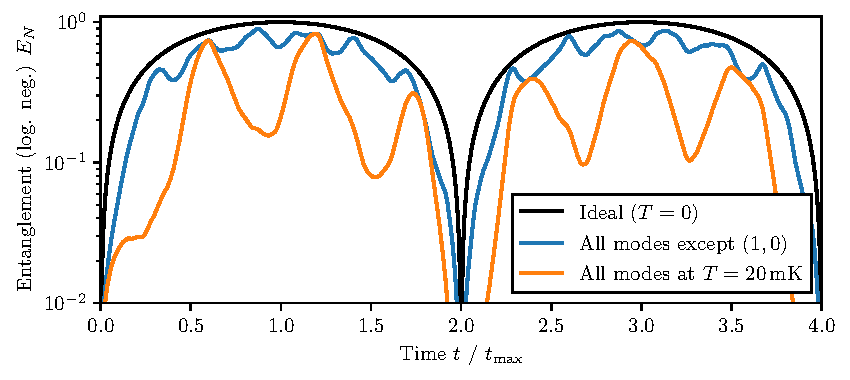
\includegraphics[width=\textwidth]{./../figures/vibrations/entanglement-multiple-modes_rs-5mm.pdf}
  \caption{Similar to \cref{fig:5:entanglement-multiple-modes} at $T=20\si{mK}$ for a slightly smaller shied with $r_s = 5\si{mm}$.}
  \label{fig:apx:entanglement-thermal-shield-rs-5mm}
\end{figure}